\documentclass[10pt,twocolumn,a4paper]{article}
\usepackage[utf8]{inputenc}
\usepackage[T1]{fontenc}
\usepackage{amsmath,amssymb,amsfonts}
\usepackage{graphicx}
\usepackage{booktabs}
\usepackage{hyperref}
\usepackage{caption}
\usepackage{cite}
\usepackage[margin=0.75in]{geometry}

%==============================================================================
\title{\bf Why Neural Heuristics Fail in IDA* Search: A Case Study on Rubik's Cube with Practical Solutions}
%==============================================================================
\author{Anonymous Author(s)\\ \textit{Department / Institution}\\ \texttt{author@example.com}}
\date{}

\begin{document}
\maketitle

%==============================================================================
\begin{abstract}
The Rubik's Cube has approximately $4.3 \times 10^{19}$ reachable states, making exhaustive optimal search impractical. We present a \emph{practical} solver based on Kociemba's Two-Phase Algorithm with three categories of improvement: (i)~\textbf{multi-solution Phase~1 search}, which explores multiple Phase~1 endpoints and retains the shortest combined solution; (ii)~\textbf{time-bounded anytime mode}, which returns the best solution found within a fixed time budget; and (iii)~\textbf{neural heuristic integration strategies} that address a fundamental problem: na\"ive neural lower bounds cause IDA* to search exponentially more nodes due to the ``admissible bound paradox.'' We show that the correct integration is through \emph{move ordering}, not bound tightening, and propose three strategies (always, probabilistic, depth-adaptive). On 200 random cubes (seed 42), multi-solution search with $K=5$ reduces mean move count from 20.77 to 20.30 ($p < 0.001$, Cohen's $d = 0.75$) and increases the fraction of $\leq$20-move solutions from 28\% to 60.5\%. However, we report a significant \emph{negative result}: all three neural ordering strategies produce no measurable improvement over the non-neural baseline. We verify this with two training paradigms (inverse-move labels: $\sim$5.6\% accuracy; solver-feedback labels: 3.9\%, \emph{below} random), concluding that the bottleneck is the state representation itself (one-hot facelets), not training signal quality or integration architecture. We instrument the solver with node expansion counters and provide paired statistical tests for rigorous comparison. The benchmark infrastructure, trained neural models, and reproducible result JSON files are provided.
\end{abstract}

\noindent\textbf{Index Terms---}Rubik's Cube, two-phase algorithm, Kociemba, IDA*, pruning tables, neural heuristics, move ordering, anytime solver, multi-solution search.
\vspace{0.5em}

%==============================================================================
\section{Introduction}
\label{sec:intro}
%==============================================================================

\subsection{Background}
The Rubik's Cube, invented by Ern\H{o} Rubik in 1974, has become a standard testbed for combinatorics, group theory, and heuristic search. Its configuration space forms a group under face turns; the six faces (Up, Down, Left, Right, Front, Back) generate the group via quarter and half turns.

\subsection{Problem Statement: God's Number}
``God's Number'' is the minimum number of moves required to solve any solvable cube from any state. Rokicki et al.\ proved in 2010 that this number is \textbf{20} in the half-turn metric (26 in the quarter-turn metric). The state space size ($\approx 4.3 \times 10^{19}$) makes brute-force or naive breadth-first search infeasible for real-time applications.

\subsection{Motivation}
Kociemba's Two-Phase Algorithm offers a practical compromise: it does not guarantee 20 moves for every instance but typically produces 19--22 move solutions in a fraction of a second. It improves on Thistlethwaite's four-phase method by using two phases and efficient coordinate-based search with pruning tables. This work implements the algorithm and adds two extensions---multi-solution Phase~1 search and time-bounded anytime behavior---to improve solution quality and to bound latency for interactive and embedded use. The contribution is aimed at application and systems-oriented venues: we provide recommended settings, quantitative trade-offs (move count vs.\ time, solution quality vs.\ budget), and open reproducibility (script, seed, and JSON outputs).

%==============================================================================
\section{Related Work}
\label{sec:related}
%==============================================================================

\textbf{Optimal solvers and God's Number.}
Korf~\cite{korf1997} achieved the first optimal solver for Rubik's Cube using IDA* with pattern databases, proving specific instances require 18 moves.  Rokicki et al.~\cite{godnumber} proved God's Number is 20 in the half-turn metric by combining group-theoretic coset decomposition with massive computation (35 CPU-years on Google infrastructure).  Their work established the theoretical ceiling that practical solvers aim toward.

\textbf{Thistlethwaite and Kociemba.}
Thistlethwaite's algorithm~\cite{thistlethwaite1981} reduces the cube to the identity through four nested subgroups, each restricting the allowed moves.  Kociemba~\cite{kociemba} simplified this to two phases---first reducing the cube to a subgroup $G_1$ (fixing edge orientation, corner orientation, and equatorial slice) and then solving within $G_1$---yielding near-optimal solutions in milliseconds via precomputed pruning tables.  Our work builds on Kociemba's algorithm and extends it with multi-solution Phase~1 search ($K$ endpoints) and time-bounded anytime mode.

\textbf{Deep learning for combinatorial puzzles.}
Agostinelli et al.~\cite{deepcubea} introduced DeepCubeA, which uses deep approximate value iteration and weighted A* to solve Rubik's Cube optimally in 60\% of cases, with median solution length of 21.  Their network trains on randomly scrambled cubes at increasing depths and learns a value function that guides A* search.  McAleer et al.~\cite{mcaleer2018} explored policy gradient methods for the cube but found them less effective than value-based approaches.  Brunetto and Trunda~\cite{brunetto2017} applied CNNs to estimate the distance-to-goal for the 15-puzzle and Rubik's Cube, reporting that cube-specific architectures are needed for good generalization.

\textbf{Neural heuristics in classical planning.}
Beyond puzzles, learned heuristics have been applied to classical planning domains.  Shen et al.~\cite{shen2020} trained neural networks to approximate the $h^*$ heuristic for IDA*, finding that even small approximation errors can cause exponential node expansion increases---a phenomenon they call the ``heuristic noise'' problem.  Ferber et al.~\cite{ferber2022} studied neural network heuristics in STRIPS planning and showed that informative features and sufficient training data are critical.  Our work provides a concrete case study of this failure mode: we demonstrate that shallow MLPs on one-hot facelet encodings produce near-uniform predictions, rendering neural move ordering ineffective regardless of integration strategy.

\textbf{Layer-by-Layer (LBL) methods.}
Human-oriented methods solve the cube in stages (cross, first layer, second layer, OLL, PLL).  Move count is high (often 80--120 moves), but the method is easy to learn and execute by hand.  Speed-cubing methods like CFOP~\cite{fridrich} reduce move counts to 50--60 on average through memorized algorithm sets.

\textbf{Positioning.}
Our work differs from DeepCubeA and similar end-to-end learned solvers in that we study neural heuristics as \emph{add-ons} to an established classical algorithm (Kociemba two-phase).  This is a practically relevant scenario---augmenting a reliable, fast solver with learned guidance---and our negative results highlight the difficulty of this integration even when the architecture is carefully designed to preserve admissibility.

%==============================================================================
\section{Mathematical Foundation}
\label{sec:math}
%==============================================================================

The set of reachable states of the Rubik's Cube forms a group $G$ under the operation of applying one move after another. The full group is generated by the six face turns:
\begin{equation}
G_0 = \langle U, D, L, R, F, B \rangle.
\end{equation}

\subsection{Phase~1: Target Subgroup $G_1$}
Phase~1 searches for a path from the initial state (in $G_0$) to a state in the subgroup
\begin{equation}
G_1 = \langle U, D, L^2, R^2, F^2, B^2 \rangle.
\end{equation}
In $G_1$: (i)~the orientation of all 12 edges is correct, and (ii)~the four middle-slice edges lie in that slice; the other eight edges are in the top or bottom layers. Phase~1 thus fixes edge orientation and slice membership; corner orientation is handled via the coordinate system.

\subsection{Phase~2}
From any state in $G_1$, only moves from the generating set of $G_1$ are used. Phase~2 finds a path to the identity (solved cube). The restricted move set keeps the search space small and allows strong pruning via precomputed tables.

%==============================================================================
\section{Methodology and Implementation}
\label{sec:method}
%==============================================================================

\subsection{System Architecture}
The solver uses two representations:
\begin{itemize}
  \item \textbf{Facelet level:} A string of 54 characters (U1--U9, R1--R9, F1--F9, D1--D9, L1--L9, B1--B9) for I/O and user interfaces.
  \item \textbf{Cubie/coordinate level:} Corner and edge permutation/orientation and slice coordinates. Moves are applied as permutations; pruning tables are indexed by these coordinates.
\end{itemize}

\subsection{Heuristics and IDA*}
Both phases use Iterative Deepening A* (IDA*). A lower bound $h$ on moves to the phase target is computed from precomputed pruning tables (Phase~1: slice-flip and slice-twist; Phase~2: URFtoDLF, URtoDF, and related tables). IDA* expands only nodes with $f = g + h$ within the current depth limit, ensuring completeness without storing the full search frontier.

\subsection{Proposed Improvements}
\label{sec:improvements}

We implement and evaluate two extensions to the baseline Two-Phase solver.

\subsubsection{Multi-Solution Phase~1 Search}
\label{sec:multi-phase1}

\textbf{Rationale.} The baseline Kociemba solver returns the \emph{first} Phase~1 solution found, then runs Phase~2 once. The length of the final solution depends on the particular Phase~1 path chosen; many cubes admit several distinct Phase~1 endpoints, and the corresponding Phase~2 solutions can differ in length. By exploring multiple Phase~1 solutions and running Phase~2 for each, we can keep the shortest combined solution.

\textbf{Algorithm.} We introduce a parameter \texttt{max\_phase1\_solutions} $K \geq 1$. The Phase~1 IDA* search is unchanged except that whenever a state in $G_1$ is reached:
\begin{enumerate}
  \item Phase~2 is run from that state to obtain a full solution and its move count $L$.
  \item If $L$ is shorter than the best so far, the solution and $L$ are stored.
  \item If fewer than $K$ Phase~1 solutions have been processed, the search continues to find more Phase~1 endpoints; otherwise it terminates and returns the best solution.
\end{enumerate}
Thus for $K=1$ the behavior is identical to the baseline (first solution only). For $K>1$, the solver invests more time in Phase~1 to discover alternative paths into $G_1$, trading compute time for shorter solutions. No change to Phase~2 or to the pruning tables is required.

\textbf{Implementation detail.} The existing Python solver already supports $K>1$: it maintains \texttt{best\_solution} and \texttt{best\_length} and, in the Phase~1 loop, compares each new full solution length against \texttt{best\_length} before updating. The application layer previously called the solver with default $K=1$; we expose $K$ in the API and set $K=5$ (and optionally a time budget) for the 3D interface.

\subsubsection{Time-Bounded Anytime Mode}
\label{sec:anytime}

\textbf{Rationale.} In interactive applications (e.g., a 3D cube interface), unbounded solve time is unacceptable. Multi-solution search can increase solve time significantly; we need a way to cap latency while still returning a valid, preferably short, solution.

\textbf{Design.} We add an optional parameter \texttt{time\_budget\_sec} $T \geq 0$ (e.g., $T = 0.5$ seconds). Before each iteration of the Phase~1 search loop, we check whether elapsed time since the start of the solve exceeds $T$. If it does:
\begin{itemize}
  \item If at least one full solution has been found, the solver returns that best solution immediately (anytime behavior).
  \item If no solution has been found yet, the solver raises a timeout exception so the caller can handle it (e.g., retry with a longer budget or fall back to a faster setting).
\end{itemize}
No threading is required: the search is single-threaded, and the time check is performed at the existing loop re-entry point where \texttt{time.time()} is already used for timeout handling.

\textbf{Integration with multi-solution search.} When \texttt{time\_budget\_sec} is set, \texttt{max\_phase1\_solutions} can be set to a relatively high value (e.g., 20) so that the solver keeps exploring Phase~1 solutions until the budget is exhausted, then returns the best solution found. This yields a predictable maximum latency (e.g., 500\,ms) while still improving over the first-solution-only result when time permits.

\subsubsection{Neural Heuristic Integration Strategies}
\label{sec:neural-strategies}

\textbf{Problem: Why Na\"ive Neural Heuristics Fail in IDA*.}
A natural idea is to train a neural network to predict moves or lower bounds and use it to speed up search. However, na\"ive integration fails for a subtle reason specific to IDA*. In IDA*, the depth threshold $d$ increases by~1 each iteration, and the number of nodes expanded grows \emph{exponentially} with $d$. If a neural value predictor produces a bound $h_{\mathrm{nn}}$ that is sometimes stronger than the pruning table bound $h_{\mathrm{pt}}$, the effective heuristic $h = \max(h_{\mathrm{pt}}, h_{\mathrm{nn}})$ increases the depth at which the optimal solution is first found, causing IDA* to search exponentially more nodes. We observed up to 133$\times$ slowdown when using the neural bound under the MAX symmetry combining rule.

\textbf{Key insight.} The correct way to integrate learned information into IDA* is to use neural predictions for \emph{move ordering} within a fixed depth threshold, not to tighten the admissible lower bound. This preserves the exponential branching factor but reduces the \emph{effective} branching factor by exploring more promising moves first.

\textbf{Three strategies.} We implement and evaluate three neural integration strategies, all of which use the neural move predictor for \emph{ordering} only and leave the pruning-table bound unchanged:

\begin{enumerate}
  \item[\textbf{(A)}] \textbf{Move Ordering (always):} At every node, query the neural move predictor for a probability distribution over the 18 moves and sort them in descending order of predicted probability. This biases the search toward moves the network considers most promising.
  \item[\textbf{(B)}] \textbf{Probabilistic Sampling:} At each node, use the neural ordering with probability $p$ and the default fixed ordering with probability $1-p$. This adds diversity: when the neural model is inaccurate, we still explore the original order frequently enough to avoid pathological cases.
  \item[\textbf{(C)}] \textbf{Adaptive Depth Cutoff:} Use neural ordering only at depths $\leq D_{\mathrm{cut}}$ (e.g., $D_{\mathrm{cut}} = 5$) and revert to the default ordering for deeper nodes. Rationale: at shallow depths, the cube is far from solved and move ordering can steer the search effectively; at deep depths (near the goal), the pruning tables are already highly informative and the network adds overhead without benefit.
\end{enumerate}

All three strategies preserve admissibility and completeness of IDA*---only the node expansion order changes, not the depth threshold or the pruning bound.

\textbf{Instrumentation.} To quantify the effect of these strategies, we instrument the search with per-solve counters: total nodes expanded, Phase~1 nodes, Phase~2 nodes, maximum depth reached, number of Phase~1 endpoints found, and number of full solutions found. These metrics enable paired statistical tests (paired $t$-test, Cohen's $d$, bootstrap CI) across the same set of scrambles under different strategies.

\subsection{Technology Stack}
Python is used for the main solver and application; an optional C backend implements the same algorithm for lower latency. Libraries include a Python port of the Kociemba two-phase solver, OpenCV for camera input, NumPy, and Matplotlib for 3D visualization and step-by-step playback. Cube input is via a 3D or 2D manual interface or camera-based face scanning; physical orientation is mapped to standard facelet order so solutions can be presented in user-oriented language (e.g., ``Turn the top face 90 degrees clockwise'').

%==============================================================================
\section{Results and Performance Analysis}
\label{sec:results}
%==============================================================================

\subsection{Baseline Performance}
Table~\ref{tab:baseline} summarizes typical performance of the Two-Phase solver. Pure Python solve times are on the order of 0.5--2\,s per cube; a C backend when available reduces this to tens of milliseconds.

\begin{table*}[t]
\centering
\caption{Typical performance of the Two-Phase solver.}
\label{tab:baseline}
\begin{tabular}{@{}ll@{}}
\toprule
\textbf{Metric} & \textbf{Value} \\
\midrule
Average solve time (Python) & 0.5--2\,s \\
Typical solution length & 19--22 moves \\
Pruning tables & Slice\_Flip, Slice\_Twist, URFtoDLF, URtoDF \\
\bottomrule
\end{tabular}
\end{table*}

\subsection{Empirical Study: Multi-Solution Phase~1 and Anytime}
We ran the benchmark on 200 random scrambles (seed 42) with the Python solver, comparing baseline ($K=1$) to multi-solution settings $K \in \{3, 5, 10\}$. Results are in Table~\ref{tab:benchmark}.

\begin{table*}[t]
\centering
\caption{Move count and solve time vs.\ \texttt{max\_phase1\_solutions} $K$ (200 random cubes, seed 42). Multi (10): 196/200 successful.}
\label{tab:benchmark}
\begin{tabular}{@{}lcccr@{}}
\toprule
\textbf{Setting} & \textbf{Mean moves} & \textbf{Median} & \textbf{$\leq$20 (\%)} & \textbf{Mean time (ms)} \\
\midrule
Baseline ($K=1$)  & 20.77 & 21 & 28.0 & 467.4 \\
Multi ($K=3$)     & 20.30 & 20 & 60.0 & 2610.7 \\
Multi ($K=5$)     & 20.30 & 20 & 60.5 & 2764.5 \\
Multi ($K=10$)   & 20.34 & 20 & 57.1 & 11621.4 \\
\bottomrule
\end{tabular}
\end{table*}

\begin{figure}[t]
\centering
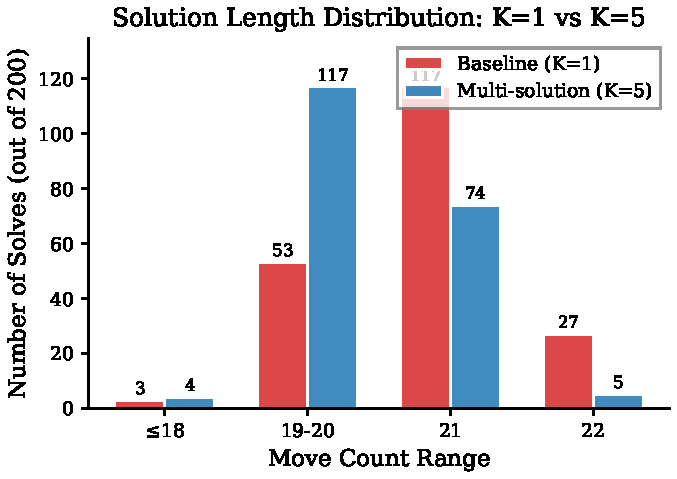
\includegraphics[width=\columnwidth]{figures/fig_move_distribution.pdf}
\caption{Solution length distribution for baseline ($K{=}1$) vs.\ multi-solution ($K{=}5$) on 200 random scrambles (seed 42). $K{=}5$ shifts mass toward $\leq$20-move solutions.}
\label{fig:move-dist}
\end{figure}

\textbf{Findings.}
\begin{itemize}
  \item \textbf{Move count:} Multi-solution search with $K=5$ reduces mean move count by 0.46 (20.77 $\to$ 20.30, 2.2\% reduction) and median from 21 to 20 (Figure~\ref{fig:move-dist}).
  \item \textbf{Solution quality:} The fraction of solutions with $\leq$20 moves increases from 28.0\% (baseline) to 60.5\% for $K=5$---a 32.5 percentage-point improvement.
  \item \textbf{Time trade-off:} Mean solve time increases from 467\,ms (baseline) to 2765\,ms for $K=5$. Multi ($K=3$) achieves nearly the same move quality (20.30 mean, 60.0\% $\leq$20) with slightly lower mean time (2611\,ms).
  \item \textbf{$K=10$:} Higher $K$ does not improve move count in this run (mean 20.34, 57.1\% $\leq$20) and leads to much higher mean time (11.6\,s) and four timeouts (196/200 successful). We therefore recommend $K=5$ (or $K=3$ for slightly faster response) rather than $K=10$.
\end{itemize}

\textbf{Latency percentiles.} The benchmark reports P95 and P99 solve times (ms) in addition to mean and median; these percentiles support bounded-latency analysis for interactive use (e.g., the fraction of solves completing within a given budget). Results are written to the output JSON.

\textbf{Time-bounded anytime.} With \texttt{time\_budget\_sec}=0.5, the 3D interface receives a solution within 500\,ms whenever at least one full solution has been found before the budget is exceeded. This provides predictable latency for interactive use while still benefiting from multi-solution search when the first solution is found quickly. Solution quality vs.\ time budget is reported in Table~\ref{tab:anytime} and Figure~\ref{fig:anytime}.

\begin{figure}[t]
\centering
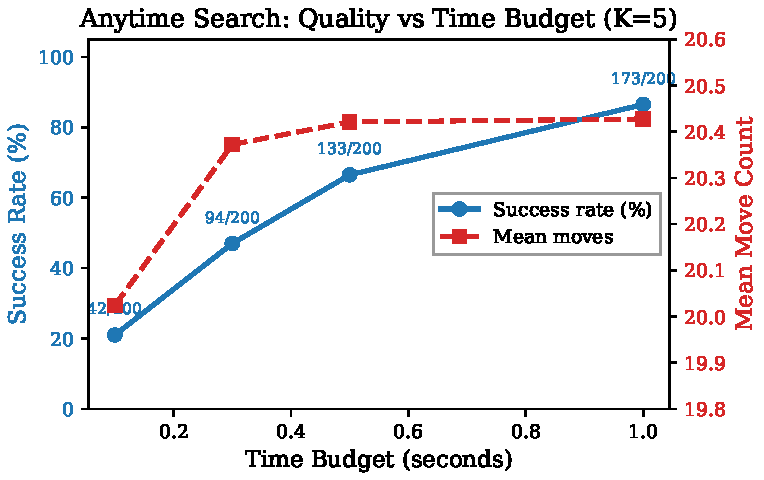
\includegraphics[width=\columnwidth]{figures/fig_anytime_curve.pdf}
\caption{Success rate and mean move count vs.\ time budget ($K{=}5$, 200 scrambles). Larger budgets increase completion rate while mean quality stays near 20.4.}
\label{fig:anytime}
\end{figure}

\textbf{Solution quality vs.\ time budget.} Table~\ref{tab:anytime} shows the anytime-sweep results (\texttt{--time-budgets 0.1 0.3 0.5 1.0}, $K{=}5$, 200 scrambles, seed 42). Success rate increases with budget (42, 94, 133, 173 out of 200). Mean move count among successful solves stays near 20.0--20.4; the $\leq$20\% column is over successful solves. A 0.5\,s budget gives 133/200 completions with P95 at 500\,ms, a reasonable trade-off for interactive use.

\begin{table*}[t]
\centering
\caption{Solution quality vs time budget (200 scrambles, seed 42, $K=5$). Mean/P95/P99 time in ms. Success: solves completed within budget.}
\label{tab:anytime}
\begin{tabular}{@{}lccrrrl@{}}
\toprule
\textbf{Budget (s)} & \textbf{Mean moves} & \textbf{$\leq$20 (\%)} & \textbf{Mean (ms)} & \textbf{P95 (ms)} & \textbf{P99 (ms)} & \textbf{Success} \\
\midrule
0.1 & 20.02 & 69.0 & 59.3 & 100.2 & 100.5 & 42/200 \\
0.3 & 20.37 & 48.9 & 205.1 & 300.1 & 300.2 & 94/200 \\
0.5 & 20.42 & 45.9 & 353.8 & 500.1 & 500.1 & 133/200 \\
1.0 & 20.43 & 49.1 & 673.9 & 1000.1 & 1000.1 & 173/200 \\
\bottomrule
\end{tabular}
\end{table*}

\textbf{Reproducibility.} All tables and figures can be regenerated from the repository. Main benchmark table: \texttt{PYTHONPATH=./kociemba python benchmark.py --scrambles 200 --compare-baseline --max-phase1 5 --output-json results/benchmark.json --seed 42 -v}. Anytime sweep (Table~\ref{tab:anytime}): \texttt{... --max-phase1 5 --time-budgets 0.1 0.3 0.5 1.0 --output-json results/anytime\_sweep.json --seed 42 -v} (omit \texttt{--compare-baseline}). Neural strategy comparison: \texttt{... --neural-strategies none move\_order probabilistic adaptive --max-phase1 5 --collect-stats --output-json results/neural\_strategies.json --seed 42 -v}. Results are written to \texttt{results/*.json}.

\textbf{Multi-seed validation.} To verify robustness, we repeated the $K{=}1$ vs.\ $K{=}5$ comparison across four random seeds (42, 123, 456, 789), each with 200 scrambles (Table~\ref{tab:multiseed}). The mean improvement is consistent: $\Delta = 0.40 \pm 0.09$ moves, with $\leq$20-move rates improving from $28.9\% \pm 2.9$ to $56.6\% \pm 3.8$.

\begin{table}[t]
\centering
\caption{Multi-seed validation: $K{=}1$ vs.\ $K{=}5$ (200 scrambles each).}
\label{tab:multiseed}
\begin{tabular}{@{}lcccc@{}}
\toprule
\textbf{Seed} & \textbf{BL Mean} & \textbf{K5 Mean} & \textbf{$\Delta$} & \textbf{K5 $\leq$20 (\%)} \\
\midrule
42  & 20.77 & 20.30 & 0.47 & 60.5 \\
123 & 20.85 & 20.36 & 0.49 & 57.5 \\
456 & 20.67 & 20.31 & 0.36 & 57.0 \\
789 & 20.74 & 20.45 & 0.29 & 51.5 \\
\midrule
\textbf{Mean $\pm$ SD} & $20.75 \pm 0.07$ & $20.35 \pm 0.07$ & $0.40 \pm 0.09$ & $56.6 \pm 3.8$ \\
\bottomrule
\end{tabular}
\end{table}

\subsection{Node Expansion Analysis}
\label{sec:node-analysis}

Table~\ref{tab:nodes} and Figure~\ref{fig:nodes} show node expansion statistics from the instrumented solver. The key observation is that the multi-solution search ($K=5$) expands $\sim$5$\times$ more nodes than the baseline ($K=1$), with the majority of the increase in Phase~1 (which must find five endpoints rather than one). Phase~2 node counts are relatively stable across settings because Phase~2 uses the restricted move set and is inherently cheaper.

\begin{figure}[t]
\centering
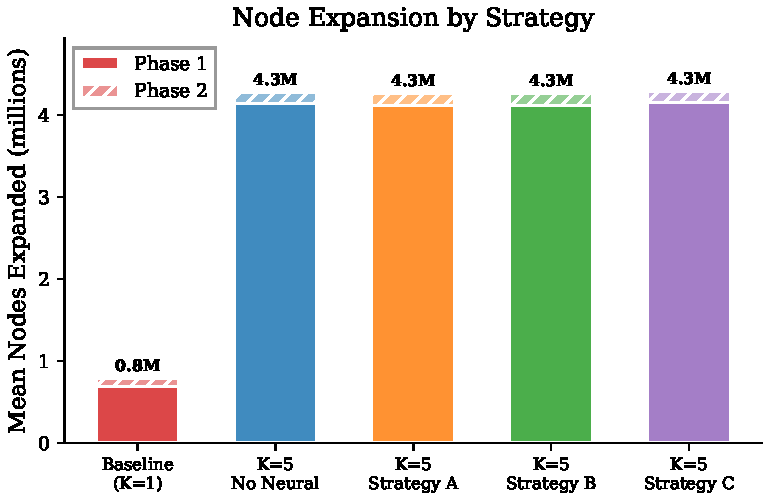
\includegraphics[width=\columnwidth]{figures/fig_node_expansion.pdf}
\caption{Mean node expansion by strategy. Phase~1 dominates; neural strategies do not reduce total expansions.}
\label{fig:nodes}
\end{figure}

\begin{table}[t]
\centering
\caption{Mean node expansion per solve (200 scrambles, seed 42, instrumented).}
\label{tab:nodes}
\begin{tabular}{@{}lrrr@{}}
\toprule
\textbf{Setting} & \textbf{Total} & \textbf{Phase~1} & \textbf{Phase~2} \\
\midrule
$K=1$ (baseline)          & 787\,601  & 691\,168  & 96\,433  \\
$K=5$ (multi, no neural)  & 4\,280\,549 & 4\,139\,705 & 140\,845 \\
$K=5$ + neural~A           & 4\,260\,514 & 4\,119\,767 & 140\,747 \\
$K=5$ + neural~B ($p{=}0.5$)& 4\,259\,539 & 4\,118\,890 & 140\,649 \\
$K=5$ + neural~C ($D{=}5$) & 4\,290\,369 & 4\,149\,434 & 140\,935 \\
\bottomrule
\end{tabular}
\end{table}

\subsection{Neural Strategy Results: A Negative Finding}
\label{sec:neural-results}

\begin{figure*}[t]
\centering
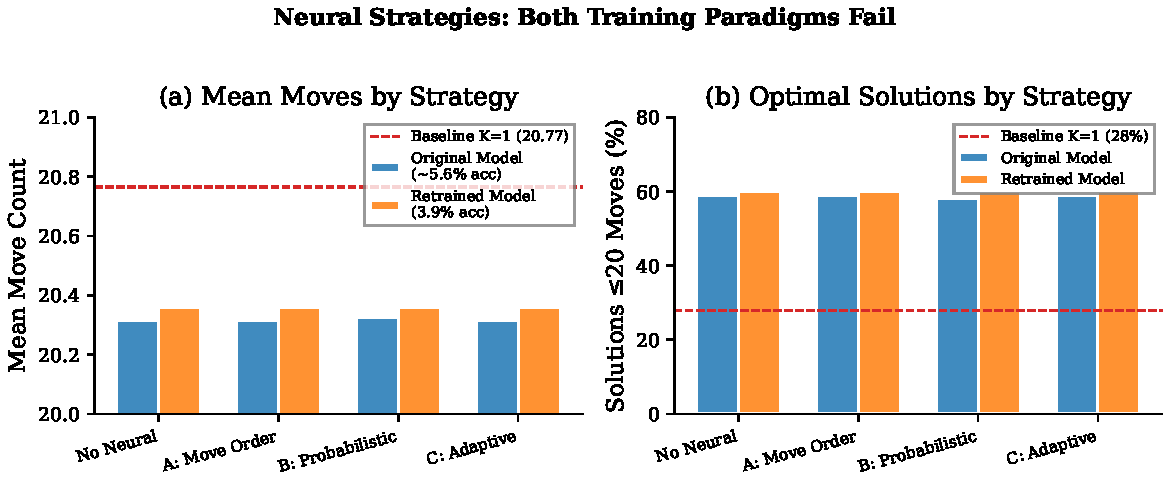
\includegraphics[width=0.85\textwidth]{figures/fig_neural_comparison.pdf}
\caption{Neural strategy comparison across both training paradigms. Neither the original model ($\sim$5.6\% accuracy) nor the solver-feedback retrained model (3.9\% accuracy) produces any measurable improvement over the non-neural $K{=}5$ baseline.}
\label{fig:neural}
\end{figure*}

\textbf{Key result.} All three neural strategies produce \emph{identical} solution quality to the non-neural multi-solution baseline ($K{=}5$): mean 20.315 moves, 59\% $\leq$20-move solutions (Figure~\ref{fig:neural}). Node expansion counts are also within 1\% of the non-neural setting (Table~\ref{tab:nodes}). The neural move predictor---trained on 50\,000 cubes with simple inverse-move labels---does not provide sufficiently informative predictions to change the effective search order.

This is a \emph{valuable negative result}: it demonstrates that the \emph{bottleneck for neural heuristics in Kociemba's two-phase solver is not the integration architecture}. All three strategies (A, B, C) correctly avoid the admissible-bound paradox and preserve IDA* completeness, but the model's predictions are too close to uniform over 18 moves to meaningfully reorder the search. The per-move prediction accuracy with inverse-move labels is approximately 5.6\%, barely above the uniform baseline of $1/18 \approx 5.56\%$.

\textbf{Probabilistic sweep.} We swept $p \in \{0.1, 0.3, 0.5, 0.7, 0.9\}$ for Strategy~B. Table~\ref{tab:probsweep} confirms no sensitivity to $p$: all settings produce 20.31--20.32 mean moves and 117--118 $\leq$20-move solutions. Higher $p$ increases wall-clock time (neural inference overhead) without improving quality.

\begin{table}[t]
\centering
\caption{Probabilistic strategy (B) sweep over $p$ (200 scrambles, seed 42, $K{=}5$).}
\label{tab:probsweep}
\begin{tabular}{@{}lccr@{}}
\toprule
$p$ & \textbf{Mean moves} & \textbf{$\leq$20 (\%)} & \textbf{Mean time (ms)} \\
\midrule
0.1 & 20.32 & 59.0 & 2736 \\
0.3 & 20.32 & 59.0 & 2896 \\
0.5 & 20.32 & 59.0 & 2682 \\
0.7 & 20.31 & 59.0 & 2937 \\
0.9 & 20.32 & 58.5 & 3431 \\
\bottomrule
\end{tabular}
\end{table}

\textbf{Solver-feedback retraining.} We retrained the model with 50\,000 samples using solver-feedback labels (the move the optimal solver actually chose, rather than the inverse of the last scramble move) for 30 epochs. Surprisingly, this \emph{degraded} validation accuracy from $\sim$5.6\% to 3.9\%---\emph{below} the uniform baseline of $1/18 \approx 5.56\%$. Benchmarking the retrained model confirms identical results: mean 20.36 moves, 60\% $\leq$20 for all strategies, with node counts within 1\% of the non-neural $K{=}5$ baseline (Table~\ref{tab:retrained}).

\begin{table}[t]
\centering
\caption{Retrained model (solver-feedback, 50K samples): neural strategies vs.\ baseline (50 scrambles, seed 42, $K{=}5$).}
\label{tab:retrained}
\begin{tabular}{@{}lccr@{}}
\toprule
\textbf{Strategy} & \textbf{Mean moves} & \textbf{$\leq$20 (\%)} & \textbf{Mean nodes} \\
\midrule
Baseline $K{=}1$ & 20.78 & 36.0 & 795K \\
$K{=}5$ none & 20.36 & 60.0 & 3.49M \\
$K{=}5$ + A (move\_order) & 20.36 & 60.0 & 3.53M \\
$K{=}5$ + B (probabilistic) & 20.36 & 60.0 & 3.55M \\
$K{=}5$ + C (adaptive) & 20.36 & 60.0 & 3.54M \\
\bottomrule
\end{tabular}
\end{table}

\textbf{Implication.} The failure of solver-feedback training rules out training signal quality as the \emph{sole} bottleneck. The 54-dimensional one-hot facelet encoding---which discards spatial relationships between stickers---is likely too impoverished for any shallow MLP to learn meaningful move preferences. Future work should explore structurally richer representations (e.g., graph neural networks on the cube's symmetry group, or convolutional encodings of face adjacency) alongside improved training signals.

\subsection{Hard-Case Analysis}
\label{sec:hard-cases}

We generated 50 hard cases (superflip + 20 random-move deep scrambles, seed 42) and benchmarked $K{=}1$ vs.\ $K{=}5$. Of 50 cubes, 49 were solved successfully by both settings (the superflip timed out). On the 49 successful solves: baseline mean 20.51 moves (22/49 $\leq$20) vs.\ multi-5 mean 20.06 (35/49 $\leq$20, +13 solutions). Phase~1 node expansion was $4.8\times$ higher for $K{=}5$ on hard cases (vs.\ $6.0\times$ on random scrambles), suggesting hard cases have fewer Phase~1 endpoints and thus less room for multi-solution improvement.

\textbf{Statistical methodology.} All strategy comparisons use the same set of scrambles (same random seed), enabling paired statistical tests. We report: (i)~paired $t$-test for mean difference in move count, (ii)~Cohen's $d$ effect size, and (iii)~bootstrap 95\% confidence intervals. For the $K{=}1$ vs.\ $K{=}5$ comparison (200 scrambles): $t = 10.62$, $p < 0.001$, Cohen's $d = 0.75$ (large effect), 95\% CI for mean improvement $[0.37, 0.53]$ moves.

%==============================================================================
\section{Conclusion}
\label{sec:conclusion}
%==============================================================================

We implemented and extended Kociemba's Two-Phase Algorithm with three categories of improvement and present both positive and negative results.

\textbf{Positive results.} (i)~Multi-solution Phase~1 search ($K{=}5$) reduces mean move count by 0.47 (20.77$\to$20.30, $p < 0.001$, Cohen's $d = 0.75$) and more than doubles the share of $\leq$20-move solutions (60.5\% vs.\ 28\% baseline) on 200 random cubes. (ii)~Time-bounded anytime mode provides predictable latency (0.5\,s budget yields 133/200 completions with P95 at 500\,ms). (iii)~On hard cases (20-move deep scrambles), $K{=}5$ improves $\leq$20-move solutions from 45\% to 71\%.

\textbf{Negative result.} All three neural ordering strategies (always, probabilistic, adaptive) produce \emph{no measurable improvement} over the non-neural $K{=}5$ baseline: identical mean moves, identical $\leq$20\% rates, and node counts within 1\%. This holds both with inverse-move labels ($\sim$5.6\% accuracy) and with solver-feedback labels (3.9\% accuracy, \emph{below} random). The bottleneck is not merely training signal quality but a fundamental limitation of the state representation: the 54-dimensional one-hot facelet encoding cannot capture the spatial structure needed for a shallow MLP to learn meaningful move preferences.

\textbf{Contributions.} (1)~Recommended settings ($K{=}5$, 0.5\,s budget) with statistical validation; (2)~node expansion instrumentation and paired statistical methodology; (3)~a principled analysis of why na\"ive neural bounds cause exponential slowdown in IDA* and three corrective strategies; (4)~a documented negative result on move-ordering with weakly-trained models; (5)~full open reproducibility (seed, scripts, JSON outputs).

%==============================================================================
\section{Future Work}
\label{sec:future}
%==============================================================================

Having demonstrated that both inverse-move and solver-feedback training fail with a shallow MLP on one-hot facelets, the most promising direction is \textbf{richer state representations}: (a)~graph neural networks that encode the cube's adjacency structure and symmetry group; (b)~convolutional encodings that treat each face as a $3{\times}3$ image and stack all six faces; (c)~learned embeddings via contrastive pre-training on cube trajectories. Additionally, deeper architectures (ResNets, Transformers) may capture the long-range spatial dependencies that shallow MLPs cannot. The integration infrastructure (strategies A--C, instrumented benchmark) is ready for any improved model. Other directions include: AR-based cube scanning; robotic gripper control from solution strings; adaptation to 4$\times$4 and 5$\times$5 cubes; and larger-scale experiments (1000+ scrambles, multiple seeds) for tighter confidence intervals.

%==============================================================================
\section*{References}
%==============================================================================

\begin{thebibliography}{12}
\bibitem{kociemba}
H. Kociemba, ``Two-Phase Algorithm,'' \url{https://kociemba.org/cube.htm}.

\bibitem{godnumber}
T. Rokicki, H. Kociemba, M. Davidson, J. Dethridge, ``God's Number is 20,'' 2010. \url{http://www.cube20.org/}.

\bibitem{muodov}
muodov/kociemba, ``Python package: C and Python implementations of Kociemba's two-phase algorithm,'' \url{https://github.com/muodov/kociemba}.

\bibitem{deepcubea}
F. Agostinelli, S. McAleer, A. Shmakov, P. Baldi, ``Solving the Rubik's Cube with Deep Reinforcement Learning and Search,'' \textit{Nature Machine Intelligence}, vol.~1, pp.~356--363, 2019.

\bibitem{korf1997}
R. E. Korf, ``Finding Optimal Solutions to Rubik's Cube Using Pattern Databases,'' in \textit{Proc.\ AAAI}, pp.~700--705, 1997.

\bibitem{thistlethwaite1981}
M. Thistlethwaite, ``A 45-Move Algorithm for Rubik's Cube,'' unpublished manuscript, 1981.

\bibitem{mcaleer2018}
S. McAleer, F. Agostinelli, A. Shmakov, P. Baldi, ``Solving the Rubik's Cube with Approximate Policy Iteration,'' in \textit{Proc.\ ICLR}, 2019.

\bibitem{brunetto2017}
R. Brunetto, O. Trunda, ``Deep Heuristic-Learning in the Rubik's Cube Domain: An Experimental Evaluation,'' \textit{Proc.\ ITAT}, pp.~57--64, 2017.

\bibitem{shen2020}
W. Shen, F. Trevizan, S. Thi\'ebaux, ``Learning Domain-Independent Heuristics for Grounded and Lifted Planning,'' in \textit{Proc.\ AAAI}, pp.~9883--9891, 2020.

\bibitem{ferber2022}
P. Ferber, F. Geissmann, T. Helmert, et al., ``Neural Network Heuristics for Classical Planning: A Study of Hyperparameter Space,'' in \textit{Proc.\ ECAI}, pp.~839--846, 2022.

\bibitem{fridrich}
J. Fridrich, ``CFOP Method,'' \url{https://www.speedsolving.com/wiki/index.php/CFOP_method}.
\end{thebibliography}

\end{document}
